\documentclass[12pt, a4 paper]{article}
% Set target color model to RGB
\usepackage[inner=2.0cm,outer=2.0cm,top=2.5cm,bottom=2.5cm]{geometry}
\usepackage{setspace}
\usepackage[rgb]{xcolor}
\usepackage{environ}
\usepackage{verbatim}
\usepackage{subcaption}
\usepackage{outlines}
\usepackage{enumitem}
\usepackage{amsgen,amsmath,amstext,amsbsy,amsopn,tikz,amssymb,tkz-linknodes}
\usepackage{fancyhdr}
\usepackage{pgfplots}
\usepackage{mathtools}
\usepackage[colorlinks=true, urlcolor=blue,  linkcolor=blue, citecolor=blue]{hyperref}
\usepackage[colorinlistoftodos]{todonotes}
\usepackage{rotating}

\linespread{1.6} % Double Line Spacing
\usetikzlibrary{arrows.meta,intersections,calc}

\hypersetup{%
pdfauthor={Vignesh Ravibaskar},%
pdfcreator={PDFLaTeX},%
pdfproducer={PDFLaTeX},%
}

% Our custom enumerate labelling, just making the outlines bold basically
\setlist[enumerate,1]{label=\textbf{\arabic*}}
\setlist[enumerate,2]{label=\textbf{({\alph*})}}
\setlist[enumerate,3]{label=\textbf{({\roman*})}}

\title{Sequences \& Series}
\author{Derek, Vignesh}
\date{2020}

\newcommand{\comm}[1]{}
\NewEnviron{answer}{\vspace{3mm} \\ \color{blue} {\BODY} \color{black}}
% \NewEnviron{answer}{\color{blue} \comm{\BODY} \color{black}} % Use this method to hide all answers

\begin{document}

\maketitle

\textbf{SEQUENCES \& SERIES [55 Marks]}

For all questions below, you may use the following standard results:
\[
 \sum_{r=1}^{n}r = \frac{1}{2}n(n+1),\: \sum_{r=1}^{n}r^2=\frac{1}{6}n(n+1)(2n+1) \textrm{ and }\sum_{r=1}^{n}r^3=\frac{1}{4}n^2{(n+1)}^2
\]
\begin{outline}[enumerate]
 \1 A geometric progression has first term \(a=\frac{1}{2}\) and common ratio \(r\). \(S_{n}\) denotes the sum of the first \(n\) terms of the progression. %Question 1

 \2 Given that the ratio \(S_{\infty}:a=3:2\), find \(r\). \hfill[1]
 \begin{answer}
  Remember that the formula for \( S_\infty \) in a Geometric Progression is given by the formula \( \dfrac{a}{1-r} \) when \( |r|<1 \)
  \begin{align*}
   S_\infty   & = \frac{a}{1-r} = \frac{3}{2}a \\
   \implies r & = \frac{1}{3}
  \end{align*}
 \end{answer}

 \2 Find the least value of \(k\) such that \(S_{k}\) is more than 99\% of \(S_{\infty}\).\hfill[3]
 \begin{answer}
  \begin{align*}
   S_k                                                & > 0.99S_\infty              \\
   \frac{a(1-r^k)}{1-r}                               & > 0.99 \cdot \frac{3}{2}a   \\
   \frac{1-{\left(\frac{1}{3}\right)}^k}{\frac{2}{3}} & > 0.99 \cdot \frac{3}{2}    \\
   \implies {\left(\frac{1}{3}\right)}^k              & < 0.01                      \\
   \implies k                                         & > -\frac{\lg{0.01}}{\lg{3}} \\
   \therefore k_{\min}                                & = 5
  \end{align*}
 \end{answer}

 \1 The sum of the first \(n\) terms of a series is given by \(S_{n}=12-12{\left(\frac{5}{6}\right)}^{n}\). %Question 2

 \2 Find \(u_{n}\). Hence, show that the series is geometric. \hfill[2]
 \begin{answer}
  Recall that the formula for \(u_n\) given \(S_n\) is \(u_n = S_n - S_{n-1} \)
  \begin{align*}
   S_n - S_{n-1} & = \left[12-12{\left(\frac{5}{6}\right)}^{n}\right] - \left[12-12{\left(\frac{5}{6}\right)}^{n-1}\right] \\
                 & = 2{\left(\frac{5}{6}\right)}^{n-1}
  \end{align*}
  The series is a geometric progression with first term 2 and common ratio \(\frac{5}{6}\)
 \end{answer}

 \2 It is given that \(u_{1}\) and \(u_{2}\) are the third and fourth term respectively of an arithmetic progression \(v_{1},v_{2},\dots \). Find \(v_{n}\) in terms of \(n\).\hfill[3]
 \begin{answer}
  \(v_3\) and \(v_4\) can be represented as \(a+2d\) and \(a+3d\) respectively where \(a\) is the first term of the AP and \(d\) is the common difference.
  \begin{align*}
   d            & =v_4-v_3=u_2-u_1 = 2-2\cdot\frac{5}{6} = \frac{1}{3}     \\
   a            & = v_3 -2d = u_1 - 2d = 2-2\cdot\frac{1}{3} = \frac{4}{3} \\
   \implies v_n & = \frac{4}{3} + \frac{1}{3}(n-1) = 1+\frac{n}{3}
  \end{align*}
 \end{answer}

 \1 A wire artist has a piece of wire of length \(L\). With one piece of wire, he can choose to make a different number of circles of different radiuses as shown: %Question 3
 \[
  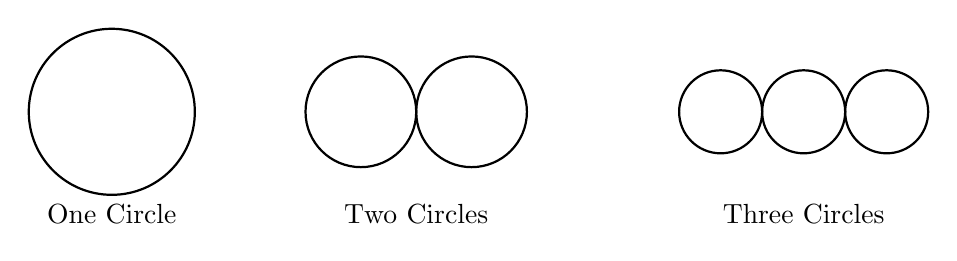
\begin{tikzpicture}
   \draw[thick] (0,0) circle (30pt);
   \draw (0,-30pt) node[below]{One Circle};
   \draw[thick] (90pt,0) circle (20pt);
   \draw[thick] (130pt,0) circle (20pt);
   \draw (110pt,-30pt) node[below]{Two Circles};
   \draw[thick] (220pt,0) circle (15pt);
   \draw[thick] (250pt,0) circle (15pt);
   \draw[thick] (280pt,0) circle (15pt);
   \draw (250pt,-30pt) node[below]{Three Circles};
  \end{tikzpicture}
 \]
 \2 Show that the area of the circles \(A_{n}\), where \(n\) denotes the number of circles formed with the wire, does not follow a geometric progression.\hfill[3]
 \begin{answer}
  Recall that the Circumference of a circle\(=2\pi r\) and the Area of a circle\(=\pi r^2\)
  \begin{align*}
   L                   & = n\cdot2\pi r                                                            \\
   A_n                 & = \pi {\left(\frac{L}{2\pi n}\right)}^2 = \frac{L^2}{4\pi n^2}            \\
   \frac{A_n}{A_{n+1}} & = \frac{L^2/4\pi n^2}{L^2/4 \pi {(n+1)}^2}={\left(\frac{n+1}{n}\right)}^2
  \end{align*}
  Since \(\frac{A_n}{A_{n+1}}\) is not a constant, \(A_n\) is not a Geometric Progression.
 \end{answer}

 \2 It is given that \(B=\frac{1}{A}\). Describe the progression \(B_{1},B_{2},\dots,B_{n},\dots \).\hfill[2]
 \begin{answer}
  Let us first find \(B_n\) in terms of \(n\)
  \begin{align*}
   B_n = \frac{1}{A_n} = \frac{4\pi}{L^2}n^2 = {\left(\frac{2\sqrt\pi}{L}n\right)}^2
  \end{align*}
  The progression is the squares of an Arithmetic Progression with first term and common difference \(\frac{2\sqrt\pi}{L}\)
 \end{answer}

 \1 Equilateral triangle \(ABC\) is inscribed in circle \(ABC\) of radius \(r\) as shown in the diagram below. A circle is then inscribed in \(\Delta ABC\), and the process continues indefinitely. %Question 4
 \[
  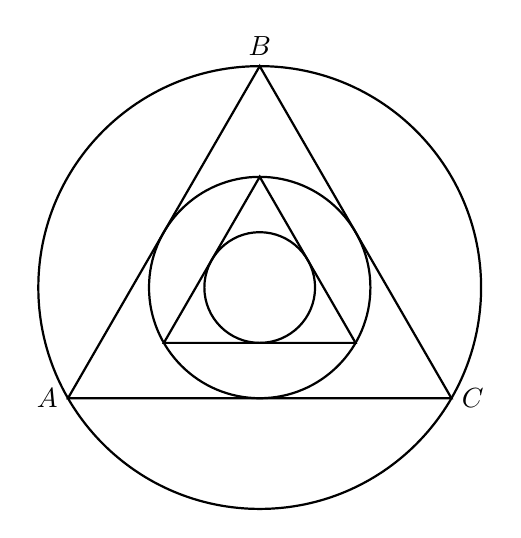
\begin{tikzpicture}
   \draw[thick] (0,0) circle (80pt);
   \draw[thick] (0,80pt) node[above]{\(B\)} -- (69.282pt,-40pt) node[right]{\(C\)} -- (-69.282pt,-40pt) node[left]{\(A\)} -- cycle;
   \draw[thick] (0,0) circle (40pt);
   \draw[thick] (0,40pt) -- (34.641pt,-20pt) -- (-34.641pt,-20pt) -- cycle;
   \draw[thick] (0,0) circle (20pt);
  \end{tikzpicture}
 \]
 \2 Show that the areas of the equilateral triangles form a geometric progression. Hence, state the sum to infinity of this geometric progression. \hfill[5]
\begin{answer}
  Let the length of the side of the 1st equilateral triangle be \(x_1\) and \(O\) be the centre of the diagram. We can find the area of this equilateral triangle \(A_1\) using the fact that \(\sphericalangle AOC = 120^{\circ}\) and \(A_1 = 3\cdot\frac{1}{2}r^2\sin(120^\circ)\) \\

  We can now find the length of each side of the triangle, \(s_1\), since \(A_1 = \frac{1}{2}s_0^2\sin60^\circ \). We can solve for \(s_1\) by equating our two expressions for \(A_1\) to get \(s_1 = \sqrt3r\) \\

  To get the radius of the inner circle, \(r_1\), we can use the fact that \(\frac{A_1}{3} = \frac{1}{2}s_1r_1\) to get \(r_1 = \frac{r}{2}\) \\

  Noticing that all the equilateral triangles are similar and the fact that the radii of the circles decreases by a factor of half at each step, the length of the sides of the \(n^{\textrm{th}}\) triangle, \(s_n\), will be \(\frac{\sqrt3}{2^{n-1}}\) \\

  Thus, the area of the \(n^{\textrm{th}}\) triangle, \(A_n = \frac{1}{2}s_n^2\sin{60^\circ} = \frac{3\sqrt3}{4^n}\). This is a geometric progression with first term \(\frac{3\sqrt3}{4}\) and common ratio \(\frac{1}{4} \implies S_\infty = \sqrt3\)
\end{answer}
 \2 An architect uses a similar design to build the tallest structure in the world constructed by cuboids stacked on top of cylinders stacked on top of cuboids and so on. Each cylindrical block is 20 storeys high and each cuboid block is 10 storeys high, where each storey is 3 metres in height. The first block, a cylinder, has a radius of 100 metres. Below is the bird's eye view of the building:
 \[
  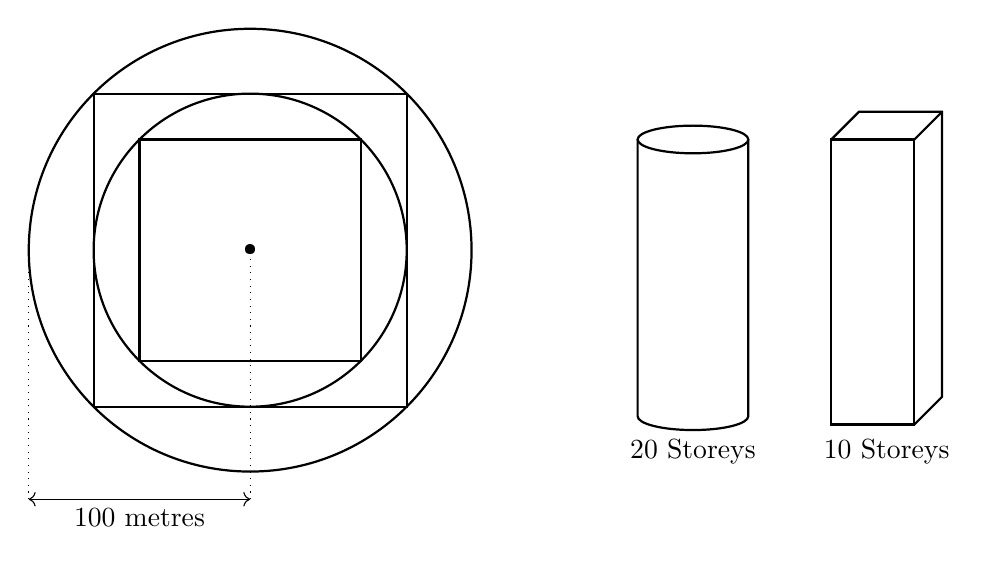
\begin{tikzpicture}
   \draw[<->] (-80pt,-90pt) -- (-40pt,-90pt)node[below]{100 metres} -- (0,-90pt);
   \draw[dotted] (-80pt,-90pt) -- (-80pt,0);
   \draw[dotted] (0pt,-90pt) -- (0,0);
   \draw[thick] (0,0) circle (80pt);
   \draw[thick] (56.5685pt,56.5685pt) -- (-56.5685pt,56.5685pt) --(-56.5685pt,-56.5685pt) -- (56.5685pt,-56.5685pt) -- cycle;
   \draw[thick] (0,0) circle (56.5685pt);
   \draw[thick] (40pt,40pt) -- (-40pt,40pt) --(-40pt,-40pt) -- (40pt,-40pt) -- cycle;
   \draw[thick] (160pt,40pt) ellipse (20pt and 5pt);
   \draw[thick] (140pt,40pt) -- (140pt,-60pt) arc (180:360:20pt and 5pt) -- (180pt,40pt);
   \draw[thick] (210pt,40pt) rectangle (240pt,-63pt);
   \draw[thick] (210pt,40pt) -- (220pt,50pt) -- (250pt,50pt) -- (250pt,-53pt) -- (240pt,-63pt);
   \draw[thick] (250pt,50pt) -- (240pt,40pt);
   \draw (160pt,-65pt) node[below]{20 Storeys};
   \draw (230pt,-65pt) node[below]{10 Storeys};
   \node at (0,0) {\textbullet};
  \end{tikzpicture}
 \]
 Due to building restrictions, the area of a block must be at least 60 m\(^2\). Find the maximum height the building can be built to.\hfill[5]
 \begin{answer}
   The length of a square inscribed in a circle is equal to \(\frac{d}{\sqrt2}\) where \(d\) is the diameter of the circle in which the square is inscribed. The subsequent circle has the same diameter as the length of the square in which it is inscribed. \\

   From this, we can glean that the area of the \(n^{\textrm{th}}\) circle, \(C_n\), can be found with the equation \(C_n = \frac{\pi\cdot200^2}{2^{n+1}}\). We can also glean that the \(n^{\textrm{th}}\) square has an area, \(S_n\), that is given by the equation \(S_n = \frac{200^2}{2^n}\). \\

   We want to find out the smallest \(n\) for which either of \(C_n\) or \(S_n\) falls below 60m\(^2\) From our G.C. we get that when \(n=10\), \(S_n < 60\) so 10 circular structures and 9 square structures would have been built up to that point. \\

   Thus, we can easily compute the height of the building to be 870m since we know that each cylindrical structure is \(20\times3=60\)m and each cuboidal structure is \(10\times3=30\)m in height.
 \end{answer}

 \1 On 1 January 2020, Jill has \$100,000 in her bank account. According to her savings plan, 2\% of her savings will be credited to this same account at the end of each month. %Question 5
 \2 Given that she spends \$5000 at the start of every month including January, find the least value of \(n\) such that she cannot finance her expenses in the \(n\)th month.\hfill[3]
 \begin{answer}
  We first will model the money left at the end of the \(n\)th month to calculate the number of months it will take for her to deplete her savings. In essence, at the end of the \(n\)th month, she does not have \$5000 left in her account.
  \begin{align*}
   \textrm{Money Left after 1st Month}     & =(100000 - 5000)\times1.02                                          \\
   \textrm{Money Left after 2nd Month}     & = [(100000-5000)\times1.02-5000]\times1.02                          \\
                                           & = 100000 \times 1.02^2 - 5000 \times 1.02^2 - 5000\times1.02        \\
   \cdots                                                                                                        \\
   \textrm{Money Left after \(n\)th Month} & = 100000 \times 1.02^n - 5000\sum_1^n{1.02^n}                       \\
                                           & = 100000 \times 1.02^n - 5000 \cdot \frac{1.02(1.02^{n}-1)}{1.02-1} \\
                                           & = 100000 \cdot 1.02^n - 255000(1.02^{n}-1)                          \\
  \end{align*}
  Now we will find when this value is less than \$5000
  \begin{align*}
   \textrm{Money Left after \(n\)th Month}  & < 5000  \\
   100000 \cdot 1.02^n - 255000(1.02^{n}-1) & < 5000  \\
   \implies n                               & > 24.14
  \end{align*}
  She will not be able to finance her expenses from the 25th month onwards.
 \end{answer}
 \2 Given instead that Jill spends \$ \(k\) at the start of every month including January, find the greatest value of \$ \(k\) such that she can afford a \$25,000 car at the end of 2020. Leave your answer to the nearest cent. \hfill[3]
 \begin{answer}
  We replace \(n\) with 24 and \$5000 with \$ \(k\) and solve for \(k\) to get our answer.
  \begin{align*}
   \textrm{Money Left after end of 24 months}                      & \geq 25000   \\
   100000 \cdot 1.02^{24} - k\cdot\frac{1.02(1.02^{24}-1)}{1.02-1} & \geq 25000   \\
   \implies k                                                      & \leq 4377.78
  \end{align*}
  She can spend a maximum of \$ \(k\) where \(k = 4377.78\) (to the nearest \textcent)
 \end{answer}
 \1 On 1 January 2020, Jack has \$5,000 in his bank account. He is looking for a savings plan to maximise his savings. Given that he spends \$200 at the start of every month including January and that interest is credit at the end of each month, what is the minimum value of \(r\), where \(r\) \% is the interest rate under the savings plan, such that Jack's balance will not go below \$4,000 by the end of 2021? Leave your answer to 3 significant figures. \hfill[5] %Question 6
 \begin{answer}
   We will model the money left at the end of the \(n\)th month to calculate the interest rate, \(r\) given that he needs to have \$4000 left after 24 months.
   \begin{align*}
     \textrm{Let } m = 1+\frac{r}{100} \\
     \textrm{Money Left after 1st Month} &= (5000-200)\cdot m \\
     \textrm{Money Left after 2nd Month} &= [(5000-200)\cdot m - 200]\cdot m \\
     \cdots \\
     \textrm{Money Left after \(n\)th Month} &= 5000\cdot m^n - 200\cdot\sum_1^n{m^n} \\
     \textrm{Money Left after 24th Month} &= 5000\cdot m^{24} - 200\cdot\frac{m(m^24-1)}{m-1} \geq 4000 \implies m \geq1.0361
   \end{align*}
   The minimum value of r is 3.61 (3 significant figures)
 \end{answer}

 \1 It is given that \(u_{r}=ar-r^2\), where \(a>0\). Given that \(\frac{1}{2k(2k+1)}\sum\limits_{r=1}^{2k}u_{r}=-\frac{13}{6}\) and \(\sum\limits_{r=k+1}^{5}u_{r}=-8\), solve for \(a\)  and \(k\) \hfill[5] %Question 7
\begin{answer}
  Notice that the sum of \(u_r\) is the combination of the sum of an arithmetic progression in \(ar + a(r+1) + a(r+2)+ \cdots \) and the combination of the sum of squares in \(-[r^2 + {(r+1)}^2 + {(r+2)}^2 + \cdots]\) \\
\begin{align*}
  \frac{1}{2k(2k+1)}\sum^{2k}_{r=1}u_r &= \frac{1}{2k(2k+1)}\left[a\frac{(2k)(2k+1)}{2} - \frac{2k(2k+1)(4k+1)}{6}\right] \\
  &= \frac{a}{2} - \frac{4k+1}{6} = -\frac{13}{6} \\
  \implies 3a-4k&=-12  \implies a = \frac{4k-12}{3} \\
  \sum^5_{r=k+1}u_r &= \sum^5_{r=1}u_r - \sum^k_{r=1}u_r \\
  &= \left[a\cdot\frac{5\times6}{2} - \frac{5\times6\times11}{6}\right] - \left[a\cdot\frac{k(k+1)}{2} - \frac{k(k+1)(2k+1)}{6}] \\
  &= \left[15\cdot\frac{4k-12}{3}-55\right] - \left[\frac{4k-12}{3}\cdot\frac{k(k+1)}{2} - \frac{k(k+1)(2k+1)}{6}\right] \\
  &= 20k-115-\frac{2k(k+1)(k-3)}{3}+\frac{k(k+1)(2k+1)}{6} \\
  \implies
\end{align*}
\end{answer}
 \1 It is given that \(u_{r}=-\frac{1+2r}{2^{r+1}(r+1)!}\). %Question 8

 \2 Show that \(u_{r}=\frac{1}{2^{r+1}(r+1)!}-\frac{1}{2^{r}(r)!}\).\hfill[2]

 \2 Hence, evaluate \(\sum\limits_{r=1}^{n}u_r\).\hfill[3]

 \2 Deduce the value of \(\sum\limits_{r=1}^{\infty}u_r\).\hfill[1]

 \1
 \2 Show that \(\cos{(k+1)}x-\cos{(k-1)x}=-2\sin{kx}\sin{x}\).\hfill[1]
\begin{answer}
  From the algebraic identity \(\cos P - \cos Q = -2\sin\frac{P+Q}{2}\sin\frac{P-Q}{2}\) we know that \(\cos{(k+1)}x-\cos{(k-1)x} = -2\sin\frac{k+1+k-1}{2}\sin\frac{k+1-k+1}{2} = -2\sin{kx}\sin x\)
\end{answer}
 \2 Find the sum of the series \(\sin{2x}+\sin{4x}+\cdots+\sin{2nx}\).\hfill[4]%Question 9
 \begin{answer}
   We rearrange the above identity to get:
   \begin{align*}
     \sin{kx} = \frac{\cos{(k-1)x}-\cos{(k+1)x}}{2\sin x}
   \end{align*}
   From this, we can simplify the given series
   \begin{align*}
     \sin{2x}+\sin{4x}+\cdots+\sin{2nx} = \frac{1}{2\sin x}[& \cos x - \cos 3x \\
     & \cos 3x - \cos 5x \\
     & \cos5x - \cos 7x \\
     & \cdots \\
     & \cos{(2n-5)x} - \cos{(2n-3)x} \\
     & \cos{(2n-3)x} - \cos{(2n-1)x} \\
     & \cos{(2n-1)x} - \cos{(2n+1)x}] \\
     &= \frac{\cos x - \cos{(2n+1)x}}{2\sin x}
   \end{align*}
 \end{answer}

 \1 Evaluate \(\sum\limits_{j=1}^{N}\mathrm{e}^{\left(\sum\limits_{r=1}^{n}u_{r}\right)j}\) given that \(u_{r}=\ln{r}\).\hfill[4]%Question 10
 \begin{answer}
  We will first evaluate the internal sum \(j\left(\sum\limits_{r=1}^{n}u_{r}\right)\)
  \begin{align*}
   (\sum\limits_{r=1}^{n}u_{r})j= j\ln\prod_{r=1}^n r = j\ln{(n!)} \\
  \end{align*}
  We can now simplify the whole sum as shown below to get our answer. Notice that we get a geometric series with first term and common ratio \(n! \) after our simplification.
  \begin{align*}
   \sum\limits_{j=1}^{N}\mathrm{e}^{\left(\sum\limits_{r=1}^{n}u_{r}\right)j} & =      \sum\limits_{j=1}^{N}\mathrm{e}^{\ln(n!) \cdot j} \\
                                                                              & = \sum\limits_{j=1}^{N}{(n!)}^j                          \\
                                                                              & = \frac{n![{(n!)}^N-1]}{n!-1}
  \end{align*}
 \end{answer}
\end{outline}
\end{document}
